\section{Implementation}
\label{sec:implementation}

\subsection{Definitions and Functions}

Future sections explore the mathematical basis and implementation of the proposed system. To provide a common reference, useful definitions and constructs are defined here.

\newcommand{\viewpoint}{\ensuremath{v}}
\newcommand{\viewpointdomain}{\ensuremath{V}}
\newcommand{\dmin}{\ensuremath{d_{\text{min}}}}
\newcommand{\dmax}{\ensuremath{d_{\text{max}}}}
\newcommand{\observation}{\ensuremath{o}}
\newcommand{\observations}[1]{\ensuremath{\boldsymbol{O}^{#1}}}
\newcommand{\pe}{\ensuremath{P(E)}}
\newcommand{\estpe}{\ensuremath{\hat{P}(E)}}
\newcommand{\ps}{\ensuremath{P(S,v)}}
\newcommand{\psge}{\ensuremath{P(S,v|E)}}
\newcommand{\estpsge}{\ensuremath{\hat{P}(S,v|E)}}
\newcommand{\psgne}{\ensuremath{P(S,v|\lnot E)}}
\newcommand{\pegs}{\ensuremath{P(E|S,v)}}
\newcommand{\pegns}{\ensuremath{P(E|\lnot S,v)}}
\newcommand{\falsepos}{\ensuremath{\varepsilon_{\text{pos}}}}
\newcommand{\falseneg}{\ensuremath{\varepsilon_{\text{neg}}}}
\newcommand{\damping}{\ensuremath{\alpha}}
\newcommand{\observability}{\ensuremath{\rho}}
\newcommand{\observabilityupdate}{\ensuremath{\eta}}
\newcommand{\state}{\ensuremath{s}}
\newcommand{\feedback}{\ensuremath{\beta}}
\newcommand{\params}[1]{\ensuremath{\boldsymbol{\theta}_{#1}}}
\newcommand{\param}[2]{\ensuremath{\theta_{#1,#2}}}
\newcommand{\epe}{\ensuremath{\text{EPE}}}
\newcommand{\vbee}{\ensuremath{\text{VBEE}}}
\newcommand{\knn}{\ensuremath{\text{KNN}}}
\newcommand{\db}{\ensuremath{\text{DB}}}
\newcommand{\initialize}[1]{\ensuremath{\operatorname{Initialize}(#1)}}
\newcommand{\estimate}[1]{\ensuremath{\operatorname{Estimate}(#1)}}
\newcommand{\integrate}[1]{\ensuremath{\operatorname{Integrate}(#1)}}
\newcommand{\update}[1]{\ensuremath{\operatorname{Update}(#1)}}
\newcommand{\query}{\ensuremath{\operatorname{Query}()}}
\newcommand{\athreshold}{\ensuremath{\tau_{\text{angle}}}}
\newcommand{\feedbackthreshold}{\ensuremath{\tau_{\beta}}}
\newcommand{\existsthreshold}{\ensuremath{\tau_{E}}}

\paragraph{Definitions}
\defitem{$\dmin$ and $\dmax$}{The minimum and maximum distances at which a map point may be considered visible to the camera.}
\defitem{$\viewpoint$}{A viewpoint in the domain $\viewpoint \in \mathbb{S}^2 \times [\dmin, \dmax] \rightarrow \mathbb{R}^3$.}
\defitem{$\observation$}{An observation of a map point defined as $\observation = (\viewpoint, \state)$, where $\viewpoint$ is the viewpoint and $\state \in \{0.0, 1.0\}$ indicates whether the point was seen (1.0) or not seen (0.0) from $\viewpoint$.}
\defitem{$\observations{n}$}{A vector of $n$ observations in the form $\{\observation_0,\dots,\observation_n\}$.}
\defitem{$\pe$}{The probability that the map point exists.}
\defitem{$\ps$}{The probability that the map point is visible from a given viewpoint $\viewpoint$.}
\defitem{$\falseneg$}{The probability of a false negative (not observing a map point when it is actually observable).}
\defitem{$\falsepos$}{The probability of a false positive (observing a map point when it is actually unobservable).}
\defitem{$\damping$}{The damping coefficient applied to updates of $\pe$.}
\defitem{$\observability_t$}{The estimated overall observability of the map point at time $t$.}
\defitem{$\observabilityupdate$}{The damping coefficient applied to updates of $\observability$.}
\defitem{$\feedback$}{The feedback propagated from the Bayesian update step back to the observability model, calculated as $\estpe_t - \estpe_{t-1}$. Used only by the KNN precursor model (see Section~\ref{sec:observability_models}).}
\defitem{$\knn$}{An instance of the KNN observability model, a precursor to the Discrete Boundary model (see Section~\ref{sec:observability_models}).}
\defitem{$\db$}{An instance of the Discrete Boundary observability model.}
\defitem{$\vbee$}{An instance of the viewpoint-based existence estimator, which holds a reference to an observability model and performs Bayesian existence probability updates internally.}
\defitem{$\params{\knn}$}{A vector of parameters specific to the KNN model in the form $\{\param{\knn}{1},\dots,\param{\knn}{n}\}$, where $n$ is the number of parameters.}
\defitem{$\params{\db}$}{A vector of parameters for the Discrete Boundary model in the form $\{k, \text{ambiguous\_range}\}$, where $k$ is the ambiguity counter maximum and $\text{ambiguous\_range}$ controls the width of the ambiguous region's output range.}
\defitem{$\params{\vbee}$}{A vector of parameters for the viewpoint-based existence estimator in the form $\{model,\estpe_0,\damping,\observability_0,\observabilityupdate,\falseneg,\falsepos\}$, where $model$ is the observability model instance.}

\paragraph{Functions}
\defitem{$\vbee.\initialize{\params{\vbee}}$}{Initializes the viewpoint-based existence estimator, including the observability model instance.}
\defitem{$\vbee.\update{\observation}$}{Updates the estimator with a new observation $\observation$, returning the updated existence probability $\estpe$.}
\defitem{$\vbee.\query$}{Queries the estimator for the current estimate of the map point's existence probability $\estpe$.}
\defitem{$\db.\initialize{\params{\db}}$}{Initializes the Discrete Boundary model with parameters $\params{\db}$.}
\defitem{$\db.\estimate{\viewpoint}$}{Returns the Discrete Boundary model's estimated probability of seeing the map point from viewpoint $\viewpoint$, given the point exists: $\estimate{\viewpoint} = \estpsge$.}
\defitem{$\db.\integrate{\observation}$}{Integrates a new observation $\observation$ into the Discrete Boundary model's internal bin state.}
\defitem{$\knn.\initialize{\params{\knn}}$}{Initializes the KNN model (precursor) with parameters $\params{\knn}$.}
\defitem{$\knn.\estimate{\viewpoint}$}{Returns the KNN model's estimated probability of seeing the map point from viewpoint $\viewpoint$: $\estimate{\viewpoint} = \estpsge$.}
\defitem{$\knn.\integrate{\observation, \feedback}$}{Integrates a new observation $\observation$ into the KNN model's stored observation buffer, using feedback $\feedback$ to determine whether the observation is incorporated.}

\subsection{Method Overview}
\label{sec:method_overview}

To achieve the goal of estimating and refining the probability of a 3D feature's existence. The estimation uses Bayesian methods to integrate prior knowledge of 3D positions where the feature is and is not visible and new observations of the feature to determine a new probability of the feature's existence. Due to the focus of this research on KV-SLAM, the 3D features discussed are 3D visual map points, but this method is adaptable to higher order features as well.

\subsubsection{The Observability Model}

The goal of the observability model is to estimate whether a point in 3D space is visible from another point in 3D space based on previous observations. These historical observations are made up of the observer's viewpoint, and whether the point of interest was visible from that location.
In the context of KV-SLAM, these points of interest are visual landmarks

Map points are conceptualized as static, infinitesimally small points in 3D Euclidean space. Let the observability of a map point $p$ from a viewpoint $\viewpoint=\{\theta,\phi,d\} \in [0,2\pi) \times \left[-\tfrac{\pi}{2}, \tfrac{\pi}{2}\right] \times [0,\dmax)$ be represented by

\[
    \operatorname{observable}_p(\viewpoint) : V \to \{0,1\},
\]

which returns $1$ if $p$ is observed from $\viewpoint$ and $0$ otherwise.
An observation of point $p$ is then defined as $\observation_p = (\viewpoint, \state)$, where $\state \in \{0,1\}$ denotes whether the point was seen.
A set of $n$ observations is $\observations{n}_p = \{\observation_{p0}, \dots, \observation_{pn}\}$.

For illustrative purposes, later figures may use a simplified 2D representation $\viewpoint^{2D}=\{\theta,d\}$. Figure \ref{fig:global_observability_p} shows an example of such a plot.

\begin{figure}[!ht]
    \centering
    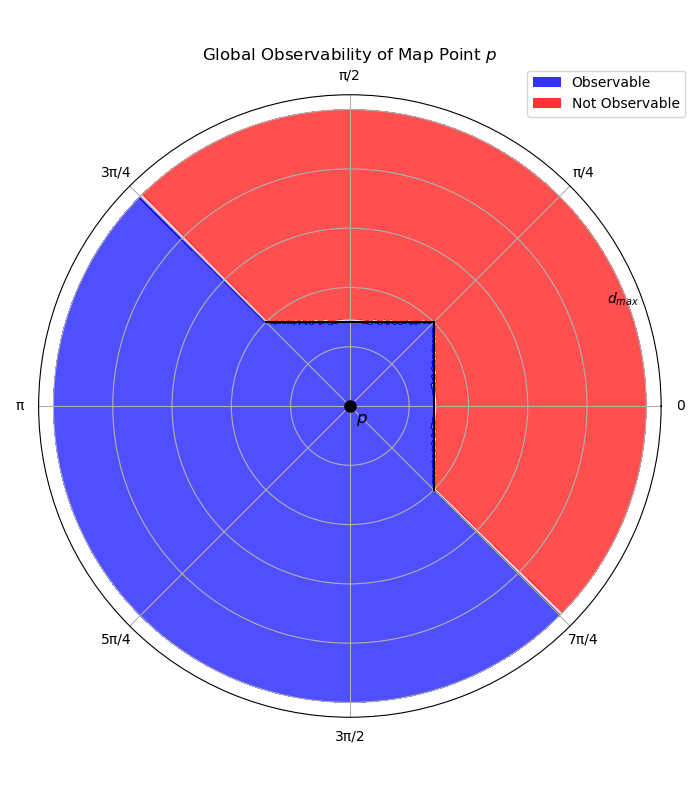
\includegraphics[width=0.7\textwidth]{resources/global_observability_p.png}
    \caption[2D Global Observability]{A 2D representation of the global observability of a map point $p$ near two orthogonal obstructions.}
    \label{fig:global_observability_p}
\end{figure}

Constructing the exact global observability surface would require infinite observations across the full domain of viewpoints, which is infeasible. To satisfy the constant-size requirement in section \ref{sec:objectives}, the observability model maintains a finite, bounded representation.

The model serves two roles:
1. Estimating $P(S,\viewpoint|E)$ from a given viewpoint.
2. Integrating new observations into its internal representation.

The objective is to minimize the total error between the model estimate and the true observability:

\[
    \int \big| \hat{P}(S,\viewpoint|E) - \operatorname{observable}_p(\viewpoint) \big| \, dV.
\]

\subsubsection{Bayesian Existence Update}

The probability of existence $\pe$ is updated with each new observation using Bayesian inference. Let $\pe_t$ denote the prior probability of existence before the observation, and $\pe_{t+1}$ the posterior after incorporating it.

\[
    \pe_{t+1} =
    \begin{cases}
        \dfrac{P(S,\viewpoint|E)\,\pe_t}{P(S,\viewpoint)}             & \text{if } \state=1, \\[1.2ex]
        \dfrac{P(\lnot S,\viewpoint|E)\,\pe_t}{P(\lnot S,\viewpoint)} & \text{if } \state=0.
    \end{cases}
\]

The marginal likelihood is

\[
    P(S,\viewpoint) = P(S,\viewpoint|E)\,\pe_t + P(S,\viewpoint|\lnot E)\,(1-\pe_t).
\]

False matches are possible when the map point does not exist. Let

\[
    \falsepos = P(S,\viewpoint|\lnot E) \approx 0,
\]

representing the false positive rate.
Assuming the model provides an estimate $\hat{P}(S,\viewpoint|E) \equiv m(\viewpoint)$, the update simplifies to

\[
    \pe_{t+1} =
    \begin{cases}
        \dfrac{m(\viewpoint)\,\pe_t}{m(\viewpoint)\,\pe_t + \falsepos(1-\pe_t)}             & \text{if } \state=1, \\[1.2ex]
        \dfrac{(1-m(\viewpoint))\,\pe_t}{(1-m(\viewpoint))\,\pe_t + (1-\falsepos)(1-\pe_t)} & \text{if } \state=0.
    \end{cases}
\]

\subsubsection{The Existence Estimation Framework}

The existence estimation framework combines an observability model with a Bayesian existence update step. A high-level view is shown in Figure \ref{fig:existence_estimation_framework}.

\begin{figure}[!ht]
    \centering
    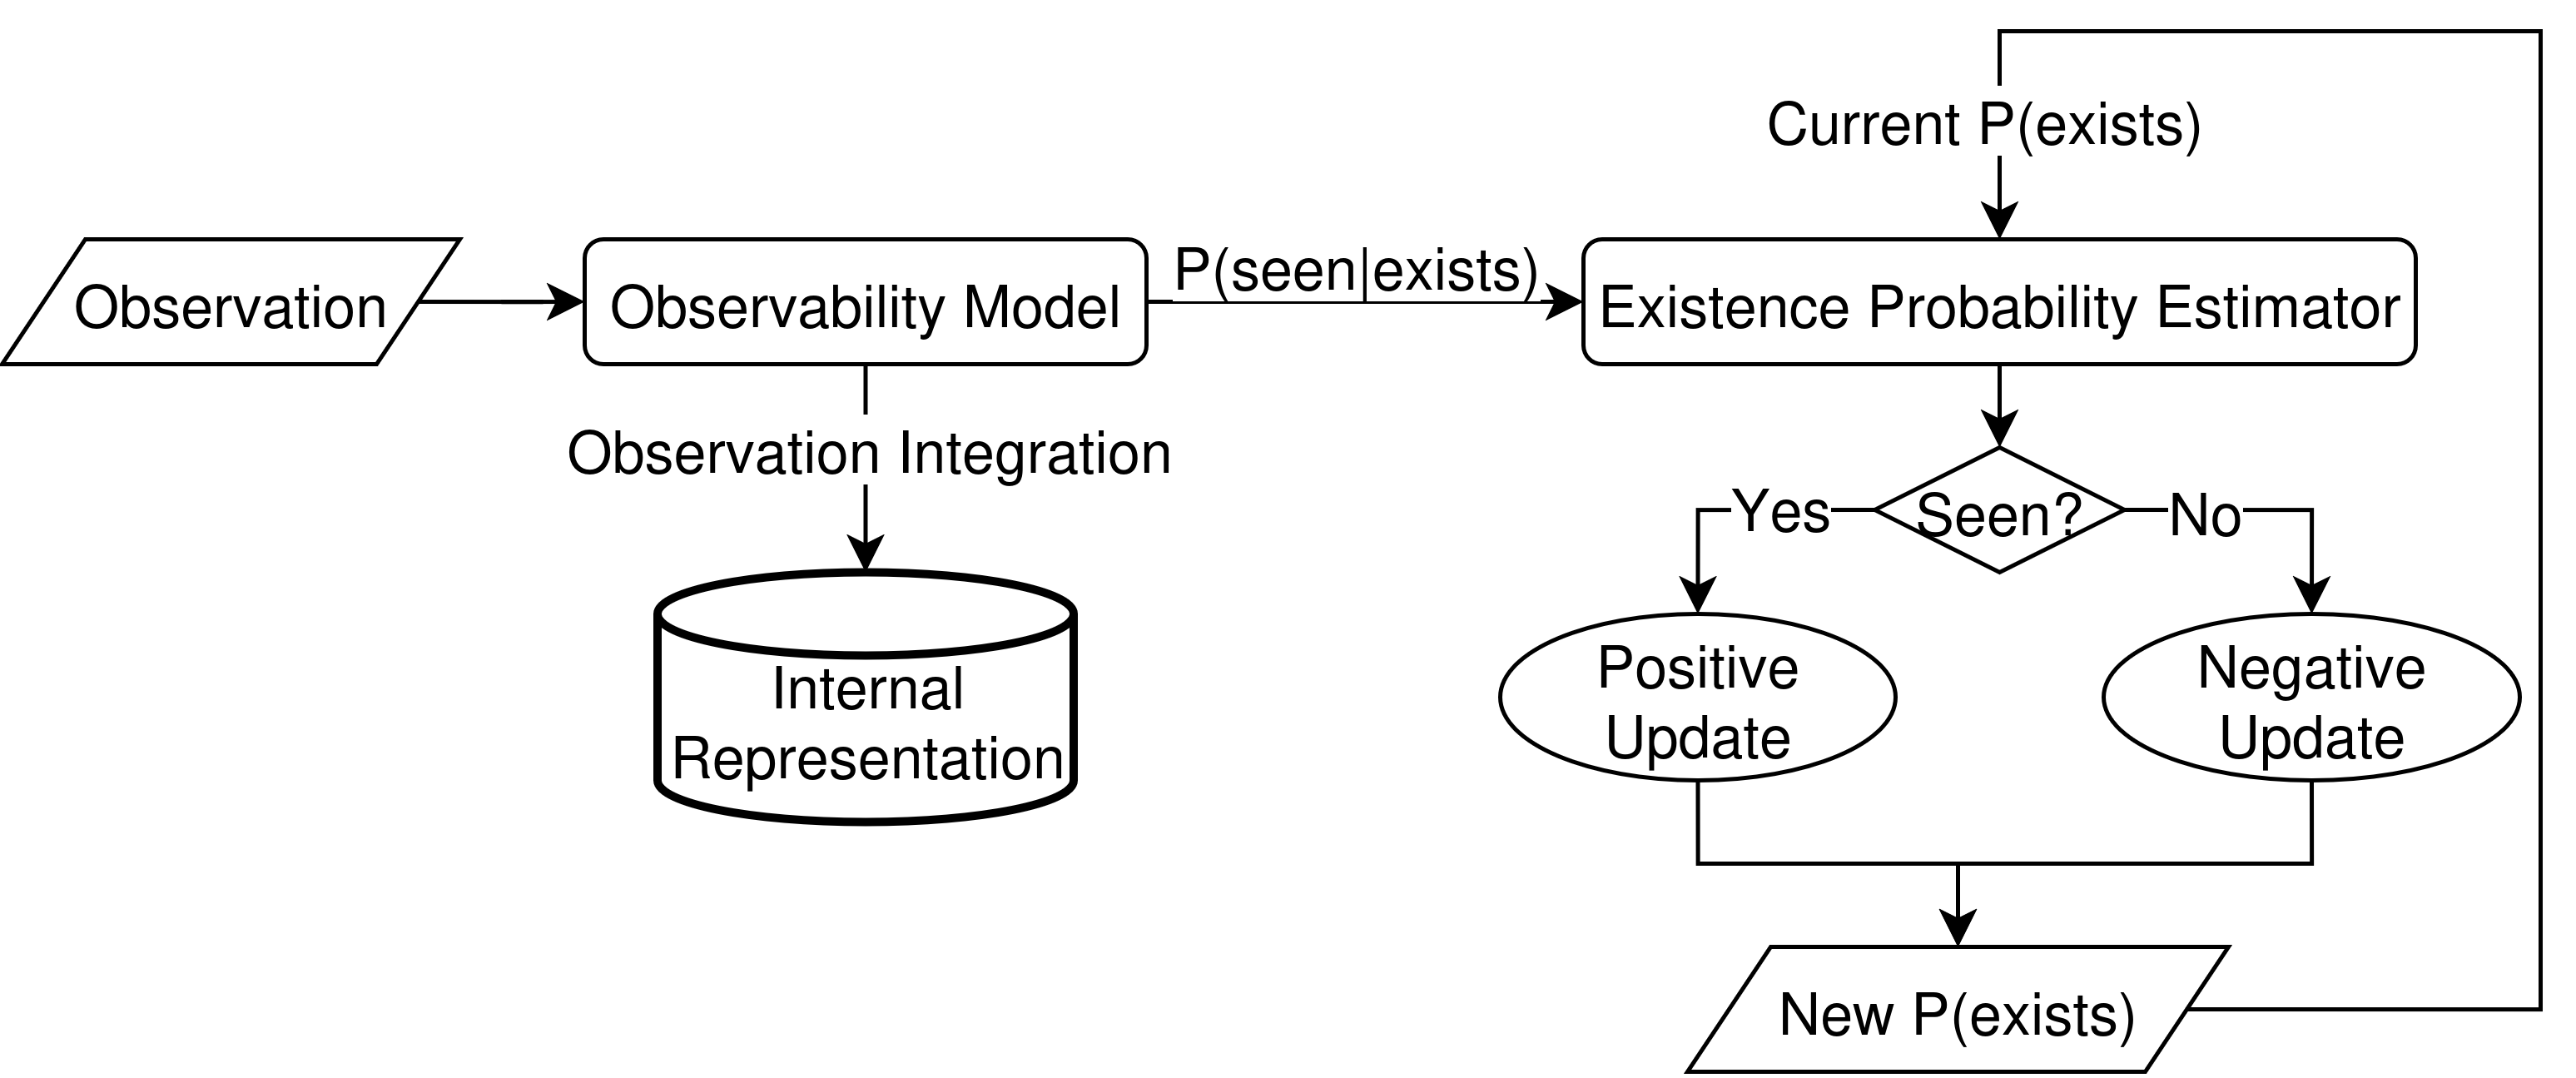
\includegraphics[width=0.7\textwidth]{resources/existence_estimation_framework.png}
    \caption[Existence Estimation Framework]{A flowchart representing the flow of data through the proposed existence estimation framework.}
    \label{fig:existence_estimation_framework}
\end{figure}

The observability model estimates $P(S,\viewpoint|E)$, the probability of observing a map point from viewpoint $\viewpoint$ given that the point exists, using historical observations. This estimate is then used to update the existence probability $\pe$ of the map point in a Bayesian manner. After the update, the new observation $\observation$ is integrated into the model's internal representation.

\subsubsection{Overall Observability}

The update above is overly sensitive in cases where a map point has historically been highly observable. For instance, if $m(\viewpoint)=1$, then a single negative observation ($\state=0$) would drive $\pe_{t+1}$ close to zero. To reduce this sensitivity, a damping coefficient $\damping \in [0,1]$ is applied:

\[
    \pe_{t+1} =
    \begin{cases}
        \damping \cdot \dfrac{m(\viewpoint)\,\pe_t}{m(\viewpoint)\,\pe_t + \falsepos(1-\pe_t)}             & \text{if } \state=1, \\[1.2ex]
        \damping \cdot \dfrac{(1-m(\viewpoint))\,\pe_t}{(1-m(\viewpoint))\,\pe_t + (1-\falsepos)(1-\pe_t)} & \text{if } \state=0.
    \end{cases}
\]

To further improve robustness, the model incorporates an overall observability parameter $\observability$, defined as the proportion of viewpoints from which the point has historically been observable. This is adaptively updated using

\[
    \observability \;\leftarrow\; \observability + \observabilityupdate \cdot \big(\state - m(\viewpoint)\big),
\]

where $\observabilityupdate$ controls the adaptation rate. In effect, $\observability$ moderates the influence of each observation, ensuring that negative evidence in highly observable regions has more weight than in rarely observable ones.

\subsection{System Implementation}

This section describes the implementation of the existence estimation framework described in section \ref{sec:method_overview}. Implementation details of the Discrete Boundary observability model and the VBEE library are provided. Pseudocode implementations of key functions are included to illustrate the implementation details of the framework.

\subsubsection{Existence Estimation Framework Implementation}

The viewpoint-based existence estimation framework is implemented as a C++ library called \texttt{libVBEE}. This library facilitates the integration of VBEE into KV-SLAM systems by providing a standardized interface for observability estimation and existence probability estimation. The library provides the \vbee{} class, which accepts an observability model through a common interface and provides functions for updating and querying the existence probability of a map point. Pseudocode for the initialization, update, and query functions is provided below.

The initialization function in Algorithm \ref{alg:vbee_init} sets up the VBEE instance with the specified parameters, including the Discrete Boundary observability model.

\begin{singlespace}
    \begin{algorithm}[H]
        \caption[VBEE Initialization]{VBEE Initialization: $\vbee.\initialize{\params{\vbee}}$}
        \label{alg:vbee_init}
        \begin{algorithmic}
            \Require $\params{\vbee}$: VBEE Parameters (includes $\params{\db}$, $\falseneg$, $\falsepos$)
            \State{\textbf{global} $p\_e, \damping, \observability, \observabilityupdate, \falseneg, \falsepos \gets \params{\vbee}$}
            \State{\textbf{global} $model \gets \db.\initialize{\params{\db}}$}
        \end{algorithmic}
    \end{algorithm}
\end{singlespace}

The update function in Algorithm \ref{alg:vbee_update} integrates a new observation, determining an updated existence probability based on the observation and the observability model's estimate. The observability model is updated with the new observation, and the overall observability is updated based on the difference between the observation's state and the model estimate.

\begin{singlespace}
    \begin{algorithm}[H]
        \caption[VBEE Update]{VBEE Update: $\vbee.\update{\observation}$}
        \label{alg:vbee_update}
        \begin{algorithmic}
            \Require $\observation$: New Observation
            \Ensure{$\estpe$: Updated Existence Probability}
            \State{$prior \gets p\_e$}
            \State{$model\_estimate \gets model.\estimate{\observation.v}$}
            \State{$posterior \gets \operatorname{BayesianUpdate}(\observation, prior, model\_estimate)$}

            \State{$weight \gets (1 - \observability) \cdot \damping$}
            \State{$p\_e \gets prior \cdot (1 - weight) + posterior \cdot weight$}

            \State{$model.\integrate{\observation}$}

            \State{$\observability \gets \observability + \observabilityupdate \cdot (\observation.s - model\_estimate)$}
            \Return{$p\_e$}
        \end{algorithmic}
    \end{algorithm}
\end{singlespace}

The query function simply returns the current existence probability $\pe$.
\subsubsection{Observability Models}
\label{sec:observability_models}

The Discrete Boundary model is implemented as the primary observability model for this system. A K-Nearest Neighbors approach was explored first and is described below to motivate the Discrete Boundary design.

\paragraph{KNN Model (Precursor)}

The KNN model estimates $\psge$ as the ratio of positive observations within the $k$ nearest neighbors of the query viewpoint. The model maintains a finite buffer of $n$ observations. The angular distance between viewpoints is also considered, as distant observations may be irrelevant. Finally, the model incorporates feedback from the existence probability estimator to decide whether or not to integrate a new observation.

The parameter vector is:
$$
    \params{\knn} = \{k, n, \athreshold, \feedbackthreshold\}
$$
where $k$ is the number of neighbors to consider, $n$ is the maximum number of stored observations, $\athreshold$ is the maximum angular distance for neighbors, and $\feedbackthreshold$ is the minimum feedback magnitude required for integration.

The estimation function is shown in Algorithm \ref{alg:knn_estimate}, returning the ratio of positive neighbors, or $0.5$ if no neighbors are found.

\begin{singlespace}
    \begin{algorithm}[H]
        \caption[KNN Observability Estimation]{KNN $\estimate{\viewpoint}$}
        \label{alg:knn_estimate}
        \begin{algorithmic}
            \Require $\observations{}_{prev}$: Stored observations
            \Require $k$, $\athreshold$: KNN parameters
            \Ensure $\estpsge$: Estimated probability of observation
            \Function{$\estimate$}{$\viewpoint$}
            \State $candidates \gets [\;]$
            \ForAll{$o \in \observations{}_{prev}$}
            \If{$\Delta\theta(o.v, \viewpoint) < \athreshold$}
            \State add $o$ to $candidates$
            \EndIf
            \EndFor
            \State \texttt{sort} $candidates$ by distance to $\viewpoint$
            \State $neighbors \gets$ first $\min(k, \texttt{length}(candidates))$
            \If{$neighbors$ is empty}
            \State \Return $0.5$
            \EndIf
            \State $seen\_count \gets$ sum of $o.s$ in $neighbors$
            \State \Return $seen\_count / \texttt{length}(neighbors)$
            \EndFunction
        \end{algorithmic}
    \end{algorithm}
\end{singlespace}

The update function (Algorithm \ref{alg:knn_update}) integrates new observations. If the buffer is not full, the observation is added. If the feedback magnitude is below $\feedbackthreshold$, the observation is ignored. Otherwise, the observation replaces the nearest inconsistent stored observation.

\begin{singlespace}
    \begin{algorithm}[H]
        \caption[KNN Model Update]{KNN $\update{o, \feedback}$}
        \label{alg:knn_update}
        \begin{algorithmic}
            \Require $\observations{}_{prev}$: Stored observations
            \Require $n$, $\feedbackthreshold$: Parameters
            \Function{$\update$}{$o, \feedback$}
            \If{$\texttt{length}(\observations{}_{prev}) < n$}
            \State add $o$
            \State \Return
            \EndIf
            \If{$|\feedback| < \feedbackthreshold$}
            \State \Return
            \EndIf
            \If{$o.s = 1$}
            \State replace nearest not-seen observation with $o$
            \Else
            \State replace nearest seen observation with $o$
            \EndIf
            \EndFunction
        \end{algorithmic}
    \end{algorithm}
\end{singlespace}

An inhert limitation with the KNN approach is its inability to exploit geometric sight-line constraints. The desire to take advantage of these constraints motivated the Discrete Boundary design described in the following section.

\paragraph{Discrete Boundary Model}

The KNN model is simple to implement and use, but it does not take advantage of geometric sight lines. If a map point can be observed from a distance d, then it is guaranteed that it can be observed from a distance < d along the same vector. The Discrete Boundary Model establishes a set of "bins" surrounding the map point, each tied to a unique direction vector. Each bin stores the radial distance to the furthest positive observation, and the closest negative observation. For each query observation, the bin whos direction vector is nearest to the queried point's direction vector is selected. Queries closer than the bin's maximum positive observation are scored with a high $\psge$. Queries more distant than the bin's furthest negative observation are scored with a low $\psge$. Queries between these values are linearly interpolated based on their relative distance to the two borders.

For simplicity, this implementation uses 20 bins, with direction vectors corresponding to the centroids of each face of an icosahedron with a vertex in the +Z direction and a face in the +X direction. This provides a consistent tiling of the sphere, so each bin covers equal angular area.

Integrating a new observation into this model first requires the selection of the appropriate bin. This can be done by identifying the direction vector with the highest dot product with the normalized vector from the map point to the viewpoint. If the observation is positive and the distance is further than that bin's current max observation distance, the max observation distance is updated to the distance between the observation and the map point. Similarly, if the observation is negative and the distance is closer than the current min non-observation distance, the bin is again updated. Bins are initialized to have 0 max observation distance and infinite minimum non-observation distance.

Because the domain of viewpoints is downsampled into a finite number of bins, it is possible for negative observations to occur at distances closer than the maximum positive distance due to environmental geometry. If a negative observation occurs at a distance less than the maximum positive distance, an "ambiguous region" is created. This is the region in which both positive and negative observations have occured, and it is given a weight based on the proportion of positive observations to all observations that occured in that region.

Querying this model is done first by identifying the bin for the given viewpoint. Once found, the region is determined. If the viewpoint's distance is greater than the maximum view distance, the query returns 0. If the viewpoint's distance is less than the minimum non-observation distance and the maximum observation distance, the query returns 1. If the observation occurs between these two values, the weighting of the ambiguous region is used to determine an estimate in the range $[0.5 - \text{ambiguous\_range}/2,\; 0.5 + \text{ambiguous\_range}/2]$, linearly mapped from the $\text{bin\_ambiguous}$ counter value.

\subsubsection{Bayesian Existence Update}
\label{sec:existence_confidence}

The Bayesian existence update computes the posterior probability $\pe$ of a map point's existence. This logic is implemented directly within the \vbee{} class and is parameterized by $\falseneg$ and $\falsepos$, now part of $\params{\vbee}$. The update takes an observation, the prior $\pe_t$, and the model estimate $\estpsge$ as inputs, and computes the posterior $\pe_{t+1}$. Algorithm \ref{alg:bayesian_update_impl} shows the implementation.

\begin{singlespace}
    \begin{algorithm}[H]
        \caption{Bayesian Update Step}
        \label{alg:bayesian_update_impl}
        \begin{algorithmic}
            \Require Observation $o = (v, s)$
            \Require Prior $\estpe_t \in [0,1]$
            \Require Model estimate $\estpsge$
            \If{$o.s = 1$}
            \State $posterior \gets \frac{\estpsge (1 - \falseneg) \cdot \estpe_t}{\estpsge (1 - \falseneg) \cdot \estpe_t + \falsepos (1 - \estpe_t)}$
            \Else
            \State $posterior \gets \frac{(1 - \estpsge (1 - \falseneg)) \cdot \estpe_t}{(1 - \estpsge (1 - \falseneg)) \cdot \estpe_t + (1 - \falsepos)(1 - \estpe_t)}$
            \EndIf
            \State \Return $posterior$
        \end{algorithmic}
    \end{algorithm}
\end{singlespace}

\subsection{Dataset Creation}
\label{sec:dataset_creation}

The Episodic Visual SLAM Dataset created for this research is a stereo visual SLAM dataset in the format of the EuRoC MAV SLAM datasets, but with extensions for episodic operation. This section details its construction and intention.

\subsubsection{Episodic Visual SLAM Datasets}

\paragraph{Hardware and Recording Setup}
The episodic datasets were recorded using a stereo camera rig in a household environment; camera calibration parameters and recording equipment specifications are documented in the dataset release.

\paragraph{Static Episodic Visual SLAM Dataset}
The static dataset consists of a sequence of trajectories recorded through an unchanged household environment, providing a baseline for measuring the effect of VBEE integration in the absence of environmental change.

\paragraph{Changing Episodic Visual SLAM Datasets}
To evaluate VBEE performance in a real-world SLAM system, a stereo visual dataset was created consisting of a series of trajectories through a household environment. No dynamic changes occur during the recording of a single trajectory, but environmental changes are introduced between trajectories, matching the episodic run modality described in section \ref{sec:background}. Figure \ref{fig:episodic_datasets} shows example images from each trajectory at roughly the same location.

\begin{figure}[H]
    \centering
    % 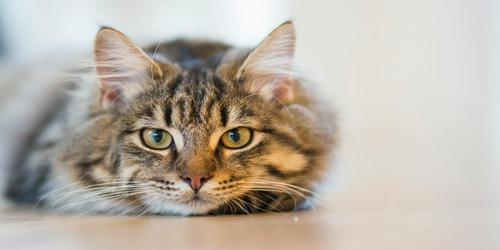
\includegraphics[width=0.8\textwidth]{resources/placeholder.jpeg}
    \caption{Example images from each trajectory of the episodic visual SLAM dataset}
    \label{fig:episodic_datasets}
\end{figure}

This dataset is intended to replicate realistic episodic SLAM operation in a household environment. Ground truth is difficult to obtain in large-scale 3D environments, so evaluation focuses on the SLAM system's ability to maintain a consistent map across multiple trajectories. LibVBEE is integrated into ORB-SLAM3, and performance is evaluated by measuring its ability to identify and remove outdated map points while preserving map consistency across episodes.

\subsection{Parameter Selection}
\label{sec:param_optimization}

The parameters of libVBEE are as follows:
$$\params{\db} = \{k, \text{ambiguous\_range}\}$$
$$\params{\vbee} = \{\estpe_0, \damping, \observability_0, \observabilityupdate, \falseneg, \falsepos\}$$
The values for these parameters were manually determined through repeated experimental trials on the episodic datasets. Both parameter sets were adjusted iteratively based on observed system behavior until stable tracking performance was achieved across multiple episodic runs. The selected parameter values are reported in Section \ref{sec:results}.

\subsection{ORB-SLAM3 Integration}
\label{sec:orb_slam3_integration}

The VBEE library is designed to be easily integrated into existing KV-SLAM systems. This section covers the integration of libVBEE into ORB-SLAM3. As discussed in section \ref{sec:orb_slam3}, ORB-SLAM3 was selected due to its wide adoption, high performance, and inclusion of several SLAM extensions which can benefit from outdated map point culling.

The original intention was to perform VBEE operations on every image frame in real-time as it passed through the SLAM system. However, these operations are time-consuming and computationally expensive, which led to a reduction in frame throughput, preventing real-time operation. Instead, the decision was made to operate on keyframes rather than frames, and to move the VBEE operations to the ends of episodic runs, acting as a post-processing step rather than a real-time update.

Several ORB-SLAM3 constructs were modified to utilize libVBEE, leading to the creation of the ORB-SLAM3 VBEE system. Implementation details split by ORB-SLAM3 construct are given below.

\subsubsection{ORB-SLAM3 Core Interface Modifications}

The VBEE library was designed to be simple to integrate into KV-SLAM systems, leading to a minimal number of changes needed to core interfaces. For ORB-SLAM3, integration of observability modeling and existence estimation can be accomplished with changes to the System class and the MapPoint class. Integration of these capabilities into RANSAC requires modifications to the MLPnPsolver, and Sim3Solver classes as well. Each of these classes is modified to have access to a global VBEE manager instance.

\begin{itemize}
    \item \textbf{System}: A function is added to be run at the end of operations to trigger VBEE post-processing.
    \item \textbf{MapPoint}: The Replace function is modified to alert the VBEE manager when two map points are successfully merged.
    \item \textbf{Sim3Solver and MLPnPsolver}:
    \begin{itemize}
        \item On construction, weights are calculated for each map point of interest based on criteria described in Section \ref{sec:orb_slam3_integration_RANSAC}.
        \item The iterate method is modified to perform selection from the weighted distribution rather than the uniform distribution.
    \end{itemize}
\end{itemize}

\subsubsection{VBEE Post-Processing Operations}

When the newly created end of operations function is called, several post-processing operations occur.

First, global bundle adjustment is performed on the active map to minimize the map error.
Next the list of new observations from the most recent operation is built using the process described in Algorithm \ref{alg:observation_creation}
\begin{singlespace}
    \begin{algorithm}[H]
        \caption{New Observation Creation}
        \label{alg:observation_creation}
        \begin{algorithmic}
            \Require $\mathcal{KF}$: New keyframes, $\mathcal{MP}$: Map points
            \Ensure $\mathcal{O}$: Set of new observations
            \State $\mathcal{O} \gets [\;]$
            \ForAll{$kf \in \mathcal{KF}$}
                \ForAll{$mp \in \mathcal{MP}$}
                    \If{$mp$ is seen in $kf$}
                        \State $v \gets kf.\text{pos} - mp.\text{pos}$
                        \State add positive observation $(mp, v)$ to $\mathcal{O}$
                    \ElsIf{$mp$ projects into the camera frame of $kf$}
                        \State $v \gets kf.\text{pos} - mp.\text{pos}$
                        \State add negative observation $(mp, v)$ to $\mathcal{O}$
                    \EndIf
                \EndFor
            \EndFor
        \end{algorithmic}
    \end{algorithm}
\end{singlespace}

The viewpoint is calculated as the difference between the keyframe and the map point's estimated positions in the map's global frame.
$$ v = KF - MP $$

It should be noted that this algorithm is extremely inefficient, and is the primary reason that VBEE operations are not attempted on a per-frame basis in real time. Many opportunities for reducing the size of the set of map points to project onto the camera frame exist, and are discussed in Section \ref{sec:future_work}.

The set of observations is then passed to the VBEE manager's update function which returns a set of map point IDs that have fallen below the threshold for map point elimination. The system then iterates through this set, and marks each map point as bad, effectively eliminating it from the map.

Finally, global bundle adjustment is run again to take advantage of any potential error reduction provided by deleting outdated map points.

\subsubsection{RANSAC Integration}
\label{sec:orb_slam3_integration_RANSAC}

RANSAC is used for relocalization and loop closing in ORB-SLAM3. The base implementation selects map points with a uniform probability of selection. The integration of VBEE into the system allows the selection to instead be weighted by the map point's probability of existence $P(E)$, or by the probability of being seen $P(S)$.

The Sim3Solver used for loop closing attempts to find a consistent relative transformation between two keyframes to establish a loop. The solver attempts to find a valid relative transformation between the two keyframes using 3D-3D correspondences. The global position of the more recent keyframe being matched is used as the viewpoint to calulate $P(S)$. While this position estimation is likely to have accumulated drift since the generation of the corresponding keyframe, this is still a valid viewpoit that can be used to calculate $P(S,v)$, which is determined as follows:

For each map point, $P(S)$ is calculated as follows:
$$
P(S)=P(S|E)P(E)+P(S|\neg E)P(\neg E)
$$

The MLPnPsolver is used for relocalization, attempting to find a valid transformation between a set of unmatched visual keypoints and the map points in ORB-SLAM3's atlas. While not localized, by definition there is no estimate for the camera's position within the global reference frame. Without an estimated camera position. Therefore, $P(E)$ is used to weight the set of candidates as opposed to $P(S,v)$.

\subsubsection{Episodic Operations Frontend}

The standard examples provided as part of ORB-SLAM3 are capable of running multiple datasets back-to-back as desired for episodic operation. However, the described episodic model allows more to be done between datasets. The episodic operating model allows us to assume a few helpful constraints will be satisfied. Oerations will start and end in the same location such as the robot's charging dock, allowing the system to have a strong localization estimate at the start of each operation. Additionally, enough time will be allowed between operations for the post-processing operations of the VBEE library to be completed, meaning VBEE operations do not compete for system resources while SLAM is actively running.

Two changes to the provided example frontends are necessary to integrate with VBEE. First, a VBEE Manager instance must be created and passed to the System class as part of the system initialization. Second, the EndEpisode function of the System class must be called at the end of each episode to trigger VBEE's post-processing.

\subsection{Experimental Setup}

The experiments defined in this section are designed to evaluate and quantify the accuracy of the observability model and the VBEE integrated SLAM system. The first experiment evaluates the Discrete Boundary observability model in isolation to determine its accuracy in estimating global observability from a finite set of observations. The remaining two experiments evaluate the performance of the VBEE integrated SLAM system, and the VBEE + RANSAC SLAM system against the unmodified baseline ORB-SLAM3 system under static and changing episodic conditions.

\subsubsection*{Experiment 1: Observability Model Prediction Quality}

The first research question defined in Section \ref{sec:rq1}

\subsubsection*{Experiment 2: VBEE Integrated SLAM Performance with Static Episodic Operations}
The goal of this experiment is to quantify the effect that VBEE integration has on KV-SLAM tracking performance under static episodic operations.

Two configurations of ORB-SLAM3 are used: the control configuration with changes made only to support episodic operations and increased keyframe generation rate, and the VBEE integrated configuration discussed in Section \ref{sec:orb_slam3_integration}. These systems are run on the static \textit{All Machine Halls} dataset discussed in Section \ref{sec:dataset_creation}.

Each system is run using the EuRoC calibration provided by the ORB-SLAM3 repository which contains camera calibrations and SLAM system parameters which have been selected experimentally \cite{mur-artalORBSLAMVersatileAccurate2015}. % Check this citation
The VBEE integrated system is run with the parameters described in Section \ref{sec:param_optimization}.

Two trajectory files are produced containing the frame trajectory and the keyframe trajectory respectively. The difference between these trajectories is discussed in Section \ref{sec:orb_slam3}, but put simply, the frame trajectory contains real-time, unoptimized pose estimates while the keyframe trajectory contains the final estimated poses of the keyframes after optimization. For each of these trajectories, the trajectory analysis tool \textit{evo} is used to produce absolute and relative pose error statistics relative to the \textit{All Machine Halls} ground truth. While evo returns several statistics for APE and RPE, the RMSE is selected as the primary measurement of trajectory error for comparison. Additional metrics are collected from the instrumentation added to ORB-SLAM3, resulting in the following being reported for each test:
\begin{itemize}
    \item $APE^{RMSE}_{KF}$ - APE RMSE for the keyframe trajectory
    \item $APE^{RMSE}_{Frame}$ - APE RMSE for the frame trajectory
    \item $RPE^{RMSE}_{KF}$ - RPE RMSE for the keyframe trajectory
    \item $RPE^{RMSE}_{Frame}$ - RPE RMSE for the frame trajectory
    \item $n_{ve}$ - The number of VBEE eliminated points at the end of the test (0 for no VBEE integration)
    \item $p_{lf}$ - The percentage of frames where the tracking system is ``lost''
    \item $n_{r}$ - The number of successful relocalizations performed during the test
    \item $n_{lc}$ - The number of successful loop closures performed during the test
\end{itemize}

Ten trials are performed for each system, with a different random seed for each trial.

\subsubsection*{Experiment 4: VBEE Integrated SLAM Performance with Changing Episodic Operations}
The goal of this experiment is to evaluate whether VBEE integration improves tracking robustness and accuracy relative to the control system when previously observed map points become outdated, as is the case in changing episodic operations.

This experiment has a construction identical to Experiment 1 in terms of system configuration, parameters, and evaluation procedure, but is run on the changing \textit{All Days} dataset described in Section \ref{sec:dataset_creation}, and evaluated against that dataset's ground truth. The same metrics are reported as in Experiment 1:
\begin{itemize}
    \item $APE^{RMSE}_{KF}$
    \item $APE^{RMSE}_{Frame}$
    \item $RPE^{RMSE}_{KF}$
    \item $RPE^{RMSE}_{Frame}$
    \item $n_{ve}$
    \item $p_{lf}$
    \item $n_{r}$
    \item $n_{lc}$
\end{itemize}

Ten trials are performed for each system with a different random seed for each trial.

\subsubsection*{Experiment 5: VBEE + RANSAC SLAM Performance with Changing Episodic Operations}
This experiment evaluates the extent to which VBEE integration combined with RANSAC weighting affects tracking robustness and accuracy relative to the control system and the unweighted VBEE integrated system under changing episodic conditions.

The configuration of the control and VBEE integrated systems are identical to Experiment 2, and because each trial is independent, the results for the control and VBEE integrated systems are reused, while the VBEE + RANSAC system is evaluated in new trials. The VBEE + RANSAC system is configured similarly to the VBEE integrated system from Experiment 2, but with RANSAC weighting enabled as discussed in Section \ref{sec:orb_slam3_integration_RANSAC}. A new metric $n_{ri}$ is added, representing the average number of RANSAC iterations needed to find sufficient inliers per successful RANSAC run.\footnote{This metric was recorded in Experiment 2 as well, but is not relevant to that experiment} The metrics reported for each test are:
 \begin{itemize}
    \item $APE^{RMSE}_{KF}$
    \item $APE^{RMSE}_{Frame}$
    \item $RPE^{RMSE}_{KF}$
    \item $RPE^{RMSE}_{Frame}$
    \item $n_{ve}$
    \item $p_{lf}$
    \item $n_{r}$
    \item $n_{lc}$
    \item $n_{ri}$
\end{itemize}